\graphicspath{{./figures/}}
\title{}
\usepackage[outputdir=latex.out]{minted}
\date{}
\begin{document}
\begin{frame}
    \titlepage
\end{frame}


\makeatletter
\newenvironment<>{btHighlight}[1][]
{\begin{onlyenv}#2\begingroup\tikzset{bt@Highlight@par/.style={#1}}\begin{lrbox}{\@tempboxa}}
{\end{lrbox}\bt@HL@box[bt@Highlight@par]{\@tempboxa}\endgroup\end{onlyenv}}

\newcommand<>\btHL[1][]{%
  \only#2{\begin{btHighlight}[#1]\bgroup\aftergroup\bt@HL@endenv}%
}
\def\bt@HL@endenv{%
  \end{btHighlight}%   
  \egroup %
}
\tikzset{
    btHLbox/.style={
        fill=red!30,outer sep=0pt,inner xsep=1pt, inner ysep=0pt, rounded corners=3pt
    },
}
\newcommand{\bt@HL@box}[2][]{%
  \tikz[#1]{%
    \pgfpathrectangle{\pgfpoint{1pt}{0pt}}{\pgfpoint{\wd #2}{\ht #2}}%
    \pgfusepath{use as bounding box}%
    \node[text width={},draw=none,anchor=base west, btHLbox, minimum height=\ht\strutbox+1pt,#1]{\raisebox{1pt}{\strut}\strut\usebox{#2}};
  }%
}

\lst@CCPutMacro
    \lst@ProcessOther {"2A}{%
      \lst@ttfamily 
         {\raisebox{2pt}{*}}% used with ttfamily
         {\raisebox{2pt}{*}}}% used with other fonts
    \@empty\z@\@empty

\lstdefinelanguage
   [x8664gas]{Assembler}     % add a "x64" dialect of Assembler
   [x86masm]{Assembler} % based on the "x86masm" dialect
   % with these extra keywords:
   {morekeywords={CDQE,CQO,CMPSQ,CMPXCHG16B,JRCXZ,LODSQ,MOVSXD,%
                  POPFQ,PUSHFQ,SCASQ,STOSQ,IRETQ,RDTSCP,SWAPGS,.TEXT,.STRING,.ASCIZ,%
                  BEQ,LW,SW,LB,SB,ADDIU,J,BEQZ,BNEZ,BNE,%
                  MOVUPD,MULPD,MOVSD,MULSD,%
                  SHLADD,MOV,CMP.LT,TBIT.NZ,BR.RET.SPTK.MANY,%
                  ADDQ,POPQ,PUSHQ,RRMOVQ,MRMOVQ,RMMOVQ,IRMOVQ,%
                  <-,LL,SC,ADDI,ADDL,VMOVDQA,ADDQ,CMPL,JB,JBE,MOVL,CLTQ,%
                  MOVW,PUSHW,MOV,ADD,SUB,INT,PUSH,MOV,ADD,REP,MOVSB,%
                  TESTQ,CMPQ,MOVL,MOVQ,ADDQ,JMPQ,XORQ,%
                  LEAQ,LEAL,LEA,RETQ,RET,POPL,POPW,PUSHL,PUSHW,%
                  LEAW,%
                  SUBQ,SYSCALL,.ASCII,CALLQ,MOVSLQ,JMP,ANDQ,SHRQ,MOVB,INCQ,TESTL,XORL,%
                  SHRL,LEAL,SARL,SUBL,IMULL,IMULQ,MOVDQU,PADDD,XORL,%
                  MOVZBL,MOVZB,SHRB,SRAL,SHRL,ANDL,%
                  CMOVNS,SRAL,SRAQ,MOVZBW,MOVZBQ,%
                  PADDW,PADDQ,MODUPS,MOVAPD,%
                  MOVL,RET,.GLOBL,%
		  PAUSE,LFENCE,JMP,%
                  },
    deletekeywords={eax,ebx,sp,si,cx,di,ds,cs,es,fs,dx,ax,bx,al,esi,ebp,ecx,rip,eip,edx,edi,rdi,esp},
    deletekeywords=[2]{size},
    alsoletter={\%},
    alsoother={()},
    emphstyle={\color{violet!50!black}},
    emph={\%rax,\%rbx,\%rcx,\%rdx,\%r8,\%r9,\%r10,\%r11,\%r12,\%r13,\%r14,\%r15,\%eax,\%ebx,\%sp,\%si,\%cx,\%di,\%ds,\%cs,\%es,\%fs,\%dx,\%ax,\%bx,\%al,\%esi,\%ebp,\%ecx,\%rip,\%eip,\%edx,\%edi,\%rdi,\%esp,\%rsp},
    %moreemph={eax,ebx,sp,si,cx,di,ds,cs,es,fs,dx,ax,bx,al,esi,ebp,ecx,rip,eip,edx,edi,rdi,esp},
    morecomment=[l]{\#},
    morecomment=[l]{\/\/},
    morecomment=[s]{/*}{*/},
    sensitive=false,
    keepspaces=true} % et

\lstalias[]{myasm}[x8664gas]{Assembler}

\lstdefinelanguage{JavaScript}{
  keywords={typeof, new, true, false, catch, function, return, null, catch, switch, var, if, in, while, do, else, case, break},
  ndkeywords={class, export, boolean, throw, implements, import, this},
  sensitive=false,
  comment=[l]{//},
  morecomment=[s]{/*}{*/},
  morestring=[b]',
  morestring=[b]"
}

\newcommand{\keywordstyle}{\sourcecodeprolight\bfseries\color{blue!30!black}}
\newcommand{\stringstyle}{\color{blue!20!black}\ttfamily}

\lstset{
    language=C,
    basicstyle=\sourcecodepro\EmptyMapping,
    escapechar=`,
    keywordstyle=\keywordstyle\EmptyMapping,
    identifierstyle=\sourcecodepro\EmptyMapping,
    numberstyle=\small\color{black!70},
    commentstyle=\color{red!60!black}\ttfamily\itshape,
    stringstyle=\color{blue!20!black}\ttfamily,
    ndkeywordstyle=\bfseries\color{blue!30!black},
    upquote=true,
}



\lstdefinestyle{medium}{
    basicstyle=\sourcecodepro\EmptyMapping\fontsize{12}{13}\selectfont,
    keywordstyle=\sourcecodepro\EmptyMapping\fontsize{12}{13}\selectfont\keywordstyle,
}

\lstdefinestyle{small}{
    basicstyle=\sourcecodepro\EmptyMapping\small,
    keywordstyle=\sourcecodepro\EmptyMapping\small\keywordstyle,
}

\lstdefinestyle{smaller}{
    basicstyle=\sourcecodepro\EmptyMapping\fontsize{11}{12}\selectfont,
    keywordstyle=\sourcecodepro\EmptyMapping\fontsize{11}{12}\selectfont\keywordstyle,
}

\lstdefinestyle{size105}{
    basicstyle=\sourcecodepro\EmptyMapping\fontsize{10.5}{11.5}\selectfont,
    keywordstyle=\sourcecodepro\EmptyMapping\fontsize{10.5}{11.5}\selectfont\keywordstyle,
}

\lstdefinestyle{size10}{
    basicstyle=\sourcecodepro\EmptyMapping\fontsize{10}{11}\selectfont,
    keywordstyle=\sourcecodepro\EmptyMapping\fontsize{10}{11}\selectfont\keywordstyle,
}

\lstdefinestyle{size9}{
    basicstyle=\sourcecodepro\EmptyMapping\fontsize{9}{10}\selectfont,
    keywordstyle=\sourcecodepro\EmptyMapping\fontsize{9}{10}\selectfont\keywordstyle,
}
\lstdefinestyle{size8}{
    basicstyle=\sourcecodepro\EmptyMapping\fontsize{8}{9}\selectfont,
    keywordstyle=\sourcecodepro\EmptyMapping\fontsize{8}{9}\selectfont\keywordstyle,
}



\lstdefinestyle{script}{
    basicstyle=\sourcecodepro\EmptyMapping\scriptsize,
    keywordstyle=\sourcecodepro\EmptyMapping\scriptsize\bfseries,
}



\section{simple control flow integrity}

\subsection{idea: checking returns?}

\begin{frame}{a simple way to check returns?}
\begin{itemize}
\item observation: places we return to usually after call instructions
    \begin{itemize}
    \item exception: `tail calls' --- we'll ignore this for now
    \end{itemize}
\vspace{.5cm}
\item we could check for one\ldots
\item replace return with:
\end{itemize}
\begin{tikzpicture}
\node[align=left,draw,very thick] {
return address $\leftarrow$ PopFromStack() \\
\textbf{if} DecodeInstruction(return address - 5) == "call thisFunction": \\
\hspace{1cm} goto return address \\
\textbf{else:} \\
\hspace{1cm} CRASH
};
\end{tikzpicture}
\end{frame}

\begin{frame}[fragile,label=simCheckRetLabel]{a simple way to check returns?}
\begin{itemize}
\item more practical: \texttt{label \$ID} instruction with encoding:
    \begin{itemize}
    \item \texttt{TWO-BYTE-OPCODE} \texttt{FOUR-BYTE-CONSTANT}
    \item (real version: can reuse some sufficiently nop-like instruction)
    \end{itemize}
\end{itemize}
\begin{tikzpicture}
\node[font=\tt,align=left,draw,very thick] (the call) {
\begin{lstlisting}[language=myasm,style=smaller]
...
    call foo
    label $0xf19279bb // random ID for function foo
...
\end{lstlisting}
};
\node[align=left,anchor=north west,draw,very thick] at ([yshift=-1cm]the call.south west) {
\begin{lstlisting}[language=myasm,style=smaller]
foo: 
...
    pop %rdx          // RDX <- return address
    cmp $0xf19279bb, 2(%rdx) 
    jne CRASH
    jmp *%rdx
\end{lstlisting}
};
\end{tikzpicture}
\end{frame}


    % FIXME: verify that it's after a call instruction
        
        % FIXME: same idea, but mark the return sites explicitly
    % FIXME: verify that it's after a call isntruction for the right function
        % FIXME: same idea, but mark the return sites explicitly

\subsubsection{versus canaries?}
\begin{frame}{looks like canaries? (1)}
    \begin{itemize}
    \item what attacks does this stop that canaries don't?
    \vspace{.5cm}
    \item<2-> ID does not need to be secret!
        \begin{itemize}
        \item<2-> assuming non-executable writeable memory, no!
        \item<2-> attacker can't write new places for return to go
        \end{itemize}
    \item<3-> avoids ``stack pivoting'' attacks
        \begin{itemize}
        \item attacker can't make stack pointer point to wrong part of stack\ldots
        \item and expect it to return differently
        \end{itemize}
    \end{itemize}
\end{frame}

\begin{frame}[fragile,label=cfiLikeCanariesP2]{looks like canaries? (2)}
    \begin{itemize}
    \item what attacks does this NOT stop that canaries don't?
    \item example: SortList can be called from \texttt{Innocent}, \\ then return from \texttt{Dangerous}
        \begin{itemize}
        \item assumption: attacker can overwrite return address at right time (running on another core? problem with sortFunc1?)
        \end{itemize}
    \end{itemize}
\begin{tikzpicture}
\node[draw,very thick,align=left] (a) {
\begin{lstlisting}[language=C++,style=smaller]
void Innocent() {
  ...
  SortList(someList1,
           sortFunc1);
  Use(someList1);
  ...
}
\end{lstlisting}
};
\node[draw,very thick,align=left,anchor=north west] at ([xshift=1cm]a.north east) (b) {
\begin{lstlisting}[language=C++,style=smaller]
void Dangerous() {
  ...
  SortList(someList2,
           sortFunc2);
  UseDangerously(someList2);
  ...
}
\end{lstlisting}
};
\end{tikzpicture}
\end{frame}


\subsection{checking VTable calls?}
    % FIXME: applying idea to calls to VTable-based function call
\begin{frame}[fragile,label=checkVTable1]{checking a VTable call}
\begin{tikzpicture}
\node[draw,very thick,align=left] (base c code) {
\begin{lstlisting}[language=C++,style=smaller]
class A { public:
  virtual void bar() { ... }
};
class B : public A { public:
  void bar() { ... }
};
void example(A *obj) {
  obj->bar();
}
\end{lstlisting}
};
\node[draw,very thick,anchor=north west,align=left] (base asm code) at ([yshift=-.25cm] base c code.south west) {
\begin{lstlisting}[language=myasm,style=smaller]
example:
  // rax <- vtable address
  movq (%rdi), %rax
  // rdx <- first vtable entry
  movq (%rax), %rax
  // call using vtable entry
  call *%rax
  ...
\end{lstlisting}
};
\begin{visibleenv}<2>
\node[draw=red,very thick,anchor=north west,align=left,font=\fontsize{12}{13}\selectfont] (warning) at ([xshift= .5cm]base asm code.north east) {
example uses VTable to call method \\
target for memory corruption attacks \\
just like return addresses \\
so, apply same strategy
};
\end{visibleenv}
\begin{visibleenv}<3->
\node[draw=red,very thick,anchor=north west,align=left] (new asm code) at ([xshift= .5cm]base asm code.north east) {
\begin{lstlisting}[language=myasm,style=smaller]
example:
  movq (%rdi), %rax
  movq (%rax), %rax
  cmpq $0xe0c5df0b, 2(%rax)
  jne CRASH
  call *%rax
  ...
\end{lstlisting}
};
\node[draw=red,very thick,anchor=south west,align=left] (new method code) at ([yshift=.5cm]new asm code.north west) {
\begin{lstlisting}[language=myasm,style=smaller]
A::bar():
  label $0xe0c5df0b
  ...
B::bar():
  label $0xe0c5df0b
  ...
\end{lstlisting}
};
\end{visibleenv}
\end{tikzpicture}
\end{frame}


\subsection{checking VTable call returns?}
    % FIXME
\begin{frame}[fragile,label=checkVTableRet1]{checking a VTable return}
\begin{tikzpicture}
\node[very thick,anchor=north west,align=left] (base asm code) {
\begin{lstlisting}[
    language=myasm,style=smaller,
    moredelim={**[is][\btHL<1->]{~1~}{~end~}},
]
example:
  movq (%rdi), %rax
  movq (%rax), %rax
  cmpq $0xe0c5df0b, 2(%rax)
  jne CRASH
  call *%rax
  ~1~label $0x64a0cfe3~end~
  ret
\end{lstlisting}
};
\node[very thick,anchor=north east,align=left] (base method code) at ([xshift=.5cm]base asm code.north west) {
\begin{lstlisting}[language=myasm,style=smaller,
    moredelim={**[is][\btHL<1->]{~1~}{~end~}},
]
A::bar():
  label $0xe0c5df0b
  ...
  ~1~pop %rdx~end~ // RDX <- return address
  ~1~cmp $0x64a0cfe3, 2(%rdx)~end~
  jne CRASH
  jmp *%rdx
B::bar():
  label $0xe0c5df0b
  ...
  ~1~pop %rdx~end~ // RDX <- return address
  ~1~cmp $0x64a0cfe3, 2(%rdx)~end~
  jne CRASH
  jmp *%rdx
\end{lstlisting}
};
\node[draw=red,very thick,anchor=north west,align=left] at ([yshift=-.5cm]base method code.south west) {
if we want to use this label-checking on the return \\
need to choose the same label for A::bar and B::bar return, too
};
\end{tikzpicture}
\end{frame}


\subsection{checking indirect function calls}
    % FIXME: trivial idea: was there a pointer?
        % well, that's not very nice\ldots
\begin{frame}[fragile,label=checkIndirectSortIntro]{calls through function pointers}
\begin{lstlisting}[language=C++,style=small]
typedef int (*CompareFnType)(const char*, const char*)
void SortFunction(const char **items, CompareFnType compare) {
    ...
    (*compare)(a, b);
    ...
}
\end{lstlisting}
\begin{itemize}
\item here: call through explicitly passed function pointer
\item want to do the same thing we did for VTable calls
    \begin{itemize}
    \item all the compare functions have the same label
    \item all the returns form compare functions have the same label
    \end{itemize}
\vspace{.5cm}
\item yes, \myemph<2->{if we can somehow label all the compare functions}
\end{itemize}
\end{frame}



\section{CFI overhead}
\begin{frame}{CFI overhead}
\begin{itemize}
\item Abadi et al's 2004 paper:
    \begin{itemize}
    \item used label-based approach
    \item 0-45\% time overhead on SPECcpu2000 benchmarks
    \item best: compression program
    \item worst: chess engine
    \end{itemize}
\item Tice et al's 2014 paper (clang-style impl, sometimes in GCC, sometimes in Clang)
    \begin{itemize}
    \item could seperately enable different parts
    \item in tests on SPECcpu 2006 benchmarks:
    \item 0--10\% slowdown for VTable dereference checks 
        \begin{itemize}
        \item but 20\% without tuning
        \end{itemize}
    \item 0-6\% for other indirect call checking
    \end{itemize}
\end{itemize}
\end{frame}


\section{what does CFI actually prevent}
\againframe<2>{cfiLikeCanariesP2}

\section{more general control flow integrity}

\subsection{concept: control flow graph}
\usetikzlibrary{calc}
\begin{frame}{concept: labels and control flow graph}
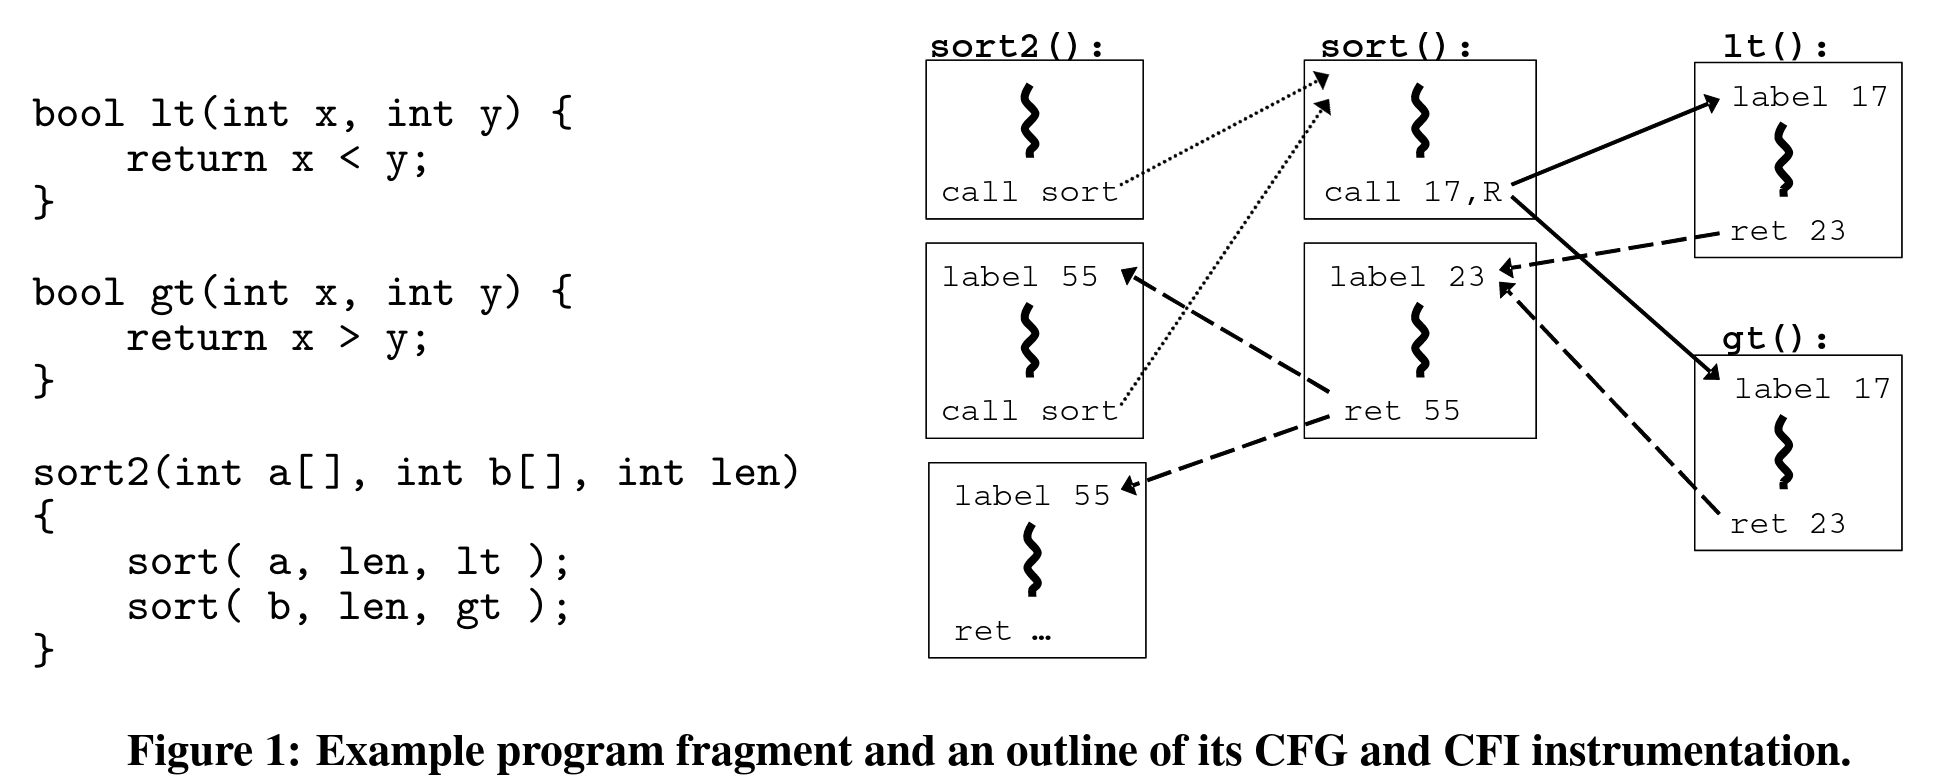
\includegraphics[width=0.7\textwidth]{../cfi/abadi-fig1}
\begin{itemize}
\item control flow graph
    \begin{itemize}
    \item nodes = blocks of code
    \item edges = \textit{potential jump/call}
    \end{itemize}
\item assigning labels: every in-edge needs to check same label at source
\end{itemize}
\imagecredit{figure from Abadi et al, ``Control-Flow Integrity: Principles, Implementations and Applications'' (CCS 2005)}
\end{frame}

 % FIXME: needs explanation of how labels assigned

\subsection{and function pointers}

\usetikzlibrary{arrows.meta}

\begin{frame}[fragile,label=tracking]{library-crossing CFGs}
\begin{tikzpicture}
\node[draw,very thick,label={north:main.c}] (mainc) {
\begin{lstlisting}[language=C++,style=script]
#include <png.h>
void ReadImageFromNetwork(
    png_structp libpng_handle,
    unsigned char *bytes,
    size_t size
) { ...  }

int main() {
    /* init libpng */
    png_structp libpng_handle = ...;
    /* tell libpng how to read image data */
    png_set_read_fn(
        libpng_handle, ...,
        ReadImageFromNetwork
    )
    ...
    /* extract "header" 
       information from image */
    png_get_IHDR(libpng_handle, ...)
    ...
}
\end{lstlisting}
};
\coordinate (base) at ([xshift=.5cm]mainc.north east);
\begin{scope}[shift=(base)]
    \tikzset{
        every node/.style={draw,align=left,font=\fontsize{10}{11}\tt\selectfont},
    }
    \node[draw,align=left,text width=1.25cm,anchor=north west] (main1) at (0,0) {
        main: \\
        ... \\
    };
    \node[draw,align=left] (set read) at (4, -1.5) {
        png\_set\_read\_fn: \\
        ... \\
        ...
    };

    \node[draw,align=left,text width=1.25cm,anchor=north west] (main2) at (0,-3) {
        ... \\
    };
    \draw[-Latex,very thick] (main1) -- (set read);
    \draw[-Latex,very thick] (set read) -- (main2);
    \node[draw,align=left] (ihdr) at (4, -4) {
        png\_get\_IHDR: \\
        ... \\
    };
    \node[draw,align=left] (readFromNet) at (5, -6) {
        ReadImage\\FromNetwork: \\
        ... 
    };
    \draw[-Latex,very thick] (main2) -- (ihdr);
    \draw[-Latex,very thick] (ihdr) -- (readFromNet);

    \begin{pgfonlayer}{bg}
    \draw[ultra thick,black!50,dotted,fill=blue!10] (-0.25,0.25) -- (1.9,0.25) -- (1.9,-5.2) -- (6.75,-5.2) --
        (6.75, -7) -- (-0.25,-7) -- cycle;
    \draw[ultra thick,black!50,dotted,fill=yellow!10] (2,-.5) -- (6.5,-.5) -- (6.5, -5) -- (2, -5) -- cycle;
    \end{pgfonlayer}
\end{scope}
\end{tikzpicture}
\end{frame}

\begin{frame}[fragile,label=imprecise]{CFGs will be imprecise}
\begin{lstlisting}[language=C++,style=smaller]
FunctionPtr p = functionA;
Example() {
  while (true) {
    ...
    if (SomethingComplicated()) {
      (*p)();
    } else if (SomethngElseComplicated()) {
      foo();
    }
    ...
  }
}
foo() {
  ...
  if (AnotherComplexThing()) {
    p = functionB;
  }
}
\end{lstlisting}
\begin{itemize}
\item can Example() call functionB()? probably not practical to tell
    \begin{itemize}
    \item need to make conservative `yes' guess
    \end{itemize}
\end{itemize}
\end{frame}


\subsection{finding function pointer values?}
\begin{frame}[fragile,label=fptrValues]{finding possible function pointer values?}
\begin{itemize}
\item given call using function pointers \\
how do we find the \textbf{legitimate} possible values?
\item one idea:
\end{itemize}
\begin{lstlisting}[language={},style=smaller,
    moredelim={**[is][\btHL<2-|handout:0>]{~2~}{~end~}},
]
for each fptr constant X: PossibleValues[X] = {X}
for each fptr ~2~variable X~end~:
    PossibleValues[X] = empty set
until PossibleValues stops changing:
    for each fptr assignment LHS=RHS:
        for ~2~each fptr variable/constant Y~end~
                ~2~that RHS could evaluate to~end~:
            PossibleValues[LHS] = Union(
                PossibleValues[LHS],
                PossibleValues[Y]
            )
\end{lstlisting}
\end{frame}




% FIXME:
\subsection{imprecision: unions, etc.}
\usetikzlibrary{arrows.meta}

\begin{frame}{labels aren't enough?}
\begin{tikzpicture}
\begin{scope}
\tikzset{
    every node/.style={align=left,draw,very thick,font=\tt\fontsize{11}{12}\selectfont},
}
\node (foo) at (0, 0){
    foo: \\
    ... \\
    check for label ??? \\
    call *p 
};

\node (bar) at (1, -5) {
    bar: \\
    ... \\
    check for label ??? \\
    call *p
};

\node (A) at (6, -2) { A: \\ label ??? };
\node (B) at (6, -3) { B: \\ label ??? };
\node (C) at (6, -4) { C: \\ label ??? };

\begin{scope}[-Latex,thick]
\draw (foo.south east) -- (A.west);
\draw (foo.south east) -- (C.west);
\draw (bar.south east) -- (B.west);
\draw (bar.south east) -- (C.west);
\end{scope}
\end{scope}
\begin{visibleenv}<2->
\node[align=left,draw=red,ultra thick,anchor=north west] at (8, 0) {
two possible fixes: \\
~ \\
make checks scan \\
for multiple labels \\
(more overhead) \\
~ \\
allow foo to call B \\
and bar to call A \\
(easier to attack)
};
\end{visibleenv}
\end{tikzpicture}
\end{frame}


\section{Clang's CFI implementation}
\begin{frame}{clang's CFI implementation}
\begin{itemize}
\item \url{https://clang.llvm.org/docs/ControlFlowIntegrity.html}
    \begin{itemize}
    \item \scriptsize also \url{https://www.usenix.org/conference/usenixsecurity14/technical-sessions/presentation/tice}
    \end{itemize}
\item only checks calls via VTables or function pointers
\item stable implementation requires libraries compiled with support
\item label information is placed in separate data structure
    \begin{itemize}
    \item \myemph<2>{looked up using function} or VTable addresses
    \end{itemize}
\item trick: keep functions in one region of memory
\end{itemize}
\end{frame}

\begin{frame}[fragile,label=indirectDiag]{clang idea for CFI indirect calls}
\begin{tikzpicture}
\node[draw, very thick, align=left] (dispatcher) {
\begin{lstlisting}[language=myasm,style=smaller]
start_funcs_with_two_string_args:
.align 8
compare_alpha:
  jmp real_compare_alpha
.align 8
run_command_with_arg:
  jmp real_run_command_with_arg
.align 8
print_two_strings:
  jmp real_print_two_strings
.align 8
move_file:
  jmp real_move_file
.align 8
compare_reverse_alpha:
  jmp real_compare_reverse_alpha
end_funcs_with_two_sting_args:
\end{lstlisting}
};
\begin{visibleenv}<1>
\node[align=left,draw=red,very thick,anchor=north west] at ([xshift=1cm]dispatcher.north east) {
functions of same type \\
placed together \\
~ \\
every func's address \\
is multiple of 8
};
\end{visibleenv}
\begin{visibleenv}<2>
\node[align=left,draw=red,very thick,anchor=north west] at ([xshift=0.5cm]dispatcher.north east) {
check pseudocode: \\
round fptr to multiple of 8 \\
\textbf{if} fptr < start or fptr > end: \\
\hspace{1cm} CRASH \\
allowed $\leftarrow$ [1,0,0,0,1] \\
\hspace{0.5cm} \textit{`mask' for compare funcs} \\
offset $\leftarrow$ fptr - start \\
\textbf{if} bit (offset/8) of allowed \\
\hspace{2.5cm}is not set: \\
\hspace{1cm} CRASH
};
\end{visibleenv}
\end{tikzpicture}
\end{frame}

\begin{frame}{clang idea for VTables}
\begin{itemize}
\item check VTable element address instead of function address
\item otherwise
    \begin{itemize}
    \item place all VTables for related classes together
    \item check start/end address for VTables
    \item bit mask indicating which VTable entries are okay for call
    \end{itemize}
\end{itemize}
\end{frame}


\section{Clang's CFI prevents?}
\begin{frame}[fragile,label=cfiPrevents]{CFI prevents?}
\begin{lstlisting}[language=C++,style=script]
class Foo { public: virtual void f() { } };
class Bar : public Foo { public: virtual void f() { g(1); } };
class Quux : public Foo { public: virtual void f() { } };
void g(int x) { if (x == 0) { danger(); } }
int h(int x) { return 0; }
int (*ptr)(int) = &h;
\end{lstlisting}
\begin{itemize}
\item with clang's CFI, which likely can end up calling \texttt{danger()}
      if an attacker can first write to arbitrary memory locations?
    \begin{itemize}
    \item A. \lstinline|(*ptr)(1);| 
    \item B. \lstinline|(*ptr)(0);| \only<2->{\myemph{if compiler thinks ptr set to g ever, yes; otherwise, no}}
    \item C. \lstinline|Foo *q = attacker_controlled(); q->f()| \only<2->{\myemph{can only call real f() methods; could call Bar::f() but how to change g's arg?}}
    \item D. \lstinline|Quux *q = attacker_controlled(); q->f()| \only<2->{\myemph{can only call real f() methods of Quux and subclasses, so can't even call Bar::f()}}
    \item E. none of these
    \end{itemize}
\end{itemize}
\end{frame}



\end{document}
